% ============================================================================
%  Comp390 — Multi-GPU / Multi-Node FHE Transformer Inference
%  Target audience: HPC researchers (not cryptographers).
%  Presenter: Halil Ibrahim Kanpak
%  Advisor:   Prof. Didem Unat, Koç University
% ============================================================================
\documentclass[aspectratio=169]{beamer}

% ---- Theme ----------------------------------------------------------------
\usetheme{metropolis}          % swap for Madrid/Berkeley if you prefer
\usepackage{appendixnumberbeamer}

% ---- Packages -------------------------------------------------------------
\usepackage[utf8]{inputenc}
\usepackage[T1]{fontenc}
\usepackage{booktabs}
\usepackage{array}
\usepackage{multirow}
\usepackage{xcolor}
\usepackage{tikz}
\usepackage{listings}
\usepackage{pgfplots}
\pgfplotsset{compat=1.18}
\usetikzlibrary{positioning,arrows.meta,shapes,fit,calc}

% ---- Colors (HPC-flavored) ------------------------------------------------
\definecolor{gpuGreen}{HTML}{76B900}      % NVIDIA green
\definecolor{hpcBlue}{HTML}{003865}       % BSC/MN5 deep blue
\definecolor{accentRed}{HTML}{C0392B}
\definecolor{mutedGray}{HTML}{555555}

\setbeamercolor{frametitle}{bg=hpcBlue,fg=white}
\setbeamercolor{title separator}{fg=gpuGreen}

% ---- Listings (for the few code snippets we show) -------------------------
\lstset{
  basicstyle=\ttfamily\scriptsize,
  keywordstyle=\color{hpcBlue}\bfseries,
  commentstyle=\color{mutedGray}\itshape,
  stringstyle=\color{accentRed},
  showstringspaces=false,
  language=C++,
  frame=single,
  framerule=0pt,
  backgroundcolor=\color{hpcBlue!5},
}

% ---- Title metadata -------------------------------------------------------
\title{Scaling Encrypted Transformer Inference\\to Multi-GPU and Multi-Node HPC}
\subtitle{An HPC perspective on a cryptographic workload}
\author{Halil İbrahim Kanpak}
\institute{Koç University — Comp390 Independent Study\\[0.3em]Advisor: Prof.\ Didem Unat}
\date{Spring 2026}

% ============================================================================
\begin{document}

% ---- Title ----------------------------------------------------------------
\begin{frame}[plain]
  \titlepage
\end{frame}

% ---- Outline --------------------------------------------------------------
\begin{frame}{Roadmap}
  \tableofcontents[hideallsubsections]
\end{frame}

% ============================================================================
\section{The problem, in HPC terms}
% ============================================================================

\begin{frame}{Why should an HPC researcher care?}
  \begin{block}{The short version}
    Every major cloud provider offers LLM inference. You send tokens, they run a
    transformer, they return tokens. \alert{They see your input in the clear.}
  \end{block}
  \pause
  \begin{block}{What privacy-preserving inference changes}
    The client encrypts its input. The server \emph{never decrypts}.
    All computation — matmuls, softmax, layer-norm — happens on ciphertexts.
  \end{block}
  \pause
  \begin{alertblock}{Why this is an HPC problem}
    The crypto makes every FLOP $10^4$–$10^6\times$ more expensive.\\
    Memory footprint per operand goes from \emph{bytes} to \emph{gigabytes}.\\
    The workload is NTT-heavy, memory-bound, and bootstrap-dominated.\\
    This \textbf{is} HPC — just with ciphertexts instead of FP16 tensors.
  \end{alertblock}
\end{frame}

% ---------------------------------------------------------------------------
\begin{frame}{The FHE workload, in one bar chart}
  \begin{center}
  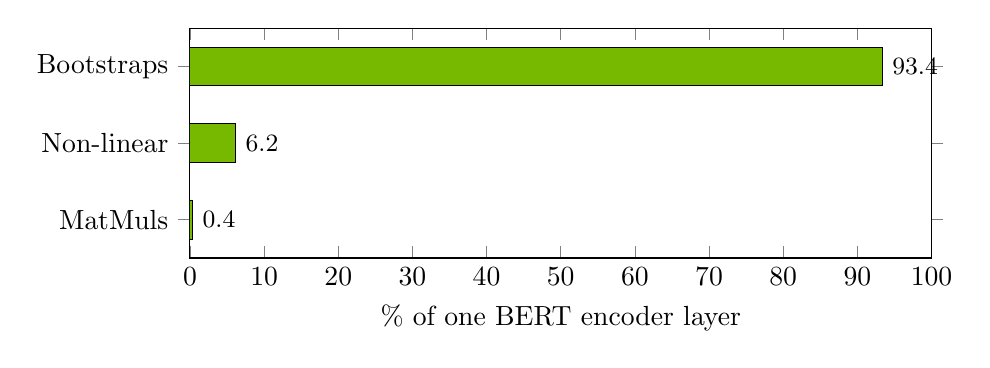
\begin{tikzpicture}
    \begin{axis}[
      xbar, bar width=14pt, width=11cm, height=4.5cm,
      enlarge y limits=0.25,
      xmin=0, xmax=100,
      xlabel={\% of one BERT encoder layer},
      symbolic y coords={MatMuls,Non-linear,Bootstraps},
      ytick=data, nodes near coords,
      nodes near coords style={font=\small}
    ]
    \addplot[fill=gpuGreen] coordinates {(93.4,Bootstraps) (6.2,Non-linear) (0.4,MatMuls)};
    \end{axis}
  \end{tikzpicture}
  \end{center}
  \vspace{-0.5em}
  \footnotesize\color{mutedGray}
  Measured on 4$\times$H100 (MareNostrum 5), $N{=}65536$, 12 heads, seq{=}16.
  \\[0.3em]
  \textbf{Takeaway:} optimizing bootstrap is optimizing the whole pipeline.
\end{frame}

% ============================================================================
\section{Background: FHE for HPC people}
% ============================================================================

\begin{frame}{The threat model — why encrypt at all?}
  \begin{columns}[T]
    \begin{column}{0.55\textwidth}
      \textbf{Today's LLM inference}
      \begin{enumerate}\small
        \item Client sends plaintext tokens.
        \item Server runs the transformer.
        \item Server returns plaintext tokens.
      \end{enumerate}
      \vspace{0.3em}
      The server sees everything. Medical records, legal briefs, trade secrets,
      source code.
    \end{column}
    \begin{column}{0.45\textwidth}
      \textbf{What we want}
      \begin{enumerate}\small
        \item Client \emph{encrypts} the input.
        \item Server runs the transformer \emph{on ciphertexts}.
        \item Server returns an encrypted result.
        \item Only the client can decrypt.
      \end{enumerate}
    \end{column}
  \end{columns}
  \vspace{0.8em}
  \begin{alertblock}{The hard part}
    \footnotesize
    Traditional encryption (AES, RSA) destroys structure: $\mathrm{Enc}(x) + \mathrm{Enc}(y)$
    is meaningless noise. We need encryption that is \textbf{homomorphic}
    — \textbf{a morphism that preserves addition and multiplication}.
  \end{alertblock}
\end{frame}

% ---------------------------------------------------------------------------
\begin{frame}{Fully Homomorphic Encryption — the one-slide intuition}
  \begin{block}{Property we need}
    $\mathrm{Dec}\big(\mathrm{Enc}(x) \oplus \mathrm{Enc}(y)\big) = x + y$ \qquad
    $\mathrm{Dec}\big(\mathrm{Enc}(x) \otimes \mathrm{Enc}(y)\big) = x \cdot y$
  \end{block}
  \vspace{0.3em}
  \begin{itemize}
    \item A \textbf{ciphertext} in CKKS is a pair of polynomials
          $(c_0, c_1) \in \mathcal{R}_q^2$ where
          $\mathcal{R}_q = \mathbb{Z}_q[X] / (X^N + 1)$.
    \item Decryption: $m + \mathrm{noise} \approx c_0 + c_1 \cdot s \pmod{q}$
          where $s$ is the secret key polynomial.
    \item Security rests on the \emph{Ring Learning-With-Errors} (RLWE) problem —
          a lattice assumption believed to resist quantum attack.
  \end{itemize}
  \vspace{0.5em}
  \begin{block}{Parameters that matter for HPC}
    \footnotesize
    \begin{tabular}{@{}ll@{}}
      $N$ (poly degree) & $2^{15}$ or $2^{16}$ for 128-bit security \\
      $\log_2 q$ (ciphertext modulus) & 1500--1800 bits, split into 30--40 RNS "limbs" \\
      Ciphertext size & 30--100 MB each \\
    \end{tabular}
  \end{block}
\end{frame}

% ---------------------------------------------------------------------------
\begin{frame}{Why is everything a polynomial? — batching}
  \begin{block}{The CKKS packing trick}
    One ciphertext encodes \textbf{not one number but a vector} of
    $N/2$ complex numbers (the "slots"). All arithmetic is element-wise.
  \end{block}
  \vspace{0.3em}
  \begin{center}
  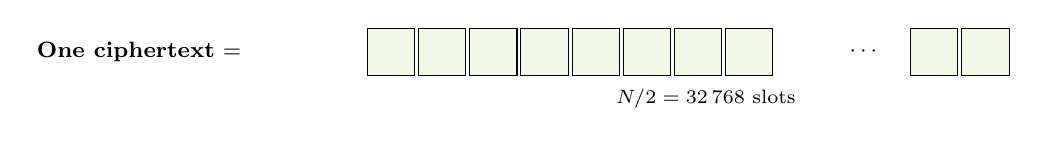
\begin{tikzpicture}[font=\footnotesize,
      slot/.style={draw,minimum width=0.6cm,minimum height=0.6cm}]
    \node (label) at (-3.2,0) {\textbf{One ciphertext} =};
    \foreach \i in {0,1,2,3,4,5,6,7}{\node[slot,fill=gpuGreen!10] at (\i*0.65,0) {};}
    \node at (6.0,0) {$\cdots$};
    \node[slot,fill=gpuGreen!10] at (6.9,0) {};
    \node[slot,fill=gpuGreen!10] at (7.55,0) {};
    \node at (4,-0.6) {\scriptsize $N/2 = 32\,768$ slots};
  \end{tikzpicture}
  \end{center}
  \vspace{0.3em}
  \begin{itemize}\small
    \item \textbf{Add / multiply:} element-wise on slots, essentially free
          (one polynomial op).
    \item \textbf{Rotate left/right across slots:} needs a \emph{Galois key};
          implemented via a ring automorphism + key-switching.
    \item To reduce a vector, you do $\log_2 N$ rotate-and-add passes.
  \end{itemize}
  \vspace{0.3em}
  \emph{This is why FHE "vectorizes": the wire format is already SIMD-over-$32\,768$-lanes.}
\end{frame}

% ---------------------------------------------------------------------------
\begin{frame}{Why rotations cost a fortune — key-switching}
  \begin{block}{Multiplication leaves the ciphertext in a "bad" key}
    \footnotesize
    $(c_0, c_1) \otimes (c_0', c_1') \to (d_0, d_1, d_2)$ — a triple under
    key $(1, s, s^2)$. Must be \textbf{key-switched} back to key $(1, s)$.
    Rotations have the same problem: after a Galois permutation, the
    ciphertext is under a \emph{different} key and must be switched back.
  \end{block}
  \pause
  \begin{block}{What key-switching does, mechanically}
    \footnotesize
    \begin{enumerate}
      \item \textbf{Decompose} one ciphertext limb into $\sim$36 digits (modulus raise).
      \item \textbf{Inner-product} each digit with the corresponding
            key component (a big RNS matrix-vector multiply).
      \item \textbf{Modulus drop} the result back to the working modulus.
    \end{enumerate}
  \end{block}
  \pause
  \begin{alertblock}{HPC consequences}
    \footnotesize
    \begin{itemize}
      \item One \textbf{key} = $\sim$1.3 GB at $N{=}65536$ (it has $\sim$36 RNS limbs).
      \item Each rotation step needs its own key.
      \item A bootstrap uses $\sim$50 different rotation steps.
      \item \textbf{48 keys $\times$ 1.3 GB = 62.4 GB} — we'll come back to this.
    \end{itemize}
  \end{alertblock}
\end{frame}

% ---------------------------------------------------------------------------
\begin{frame}{Why bootstrapping exists — the noise problem}
  \begin{block}{Every ciphertext carries an error term}
    \footnotesize
    $c_0 + c_1 \cdot s = m + e \pmod{q}$ \quad with $\|e\|$ small.
    \\
    Each multiplication makes $e$ \textbf{grow}. After a few levels, $e$
    overwhelms the message — decryption fails.
  \end{block}
  \pause
  \begin{center}
  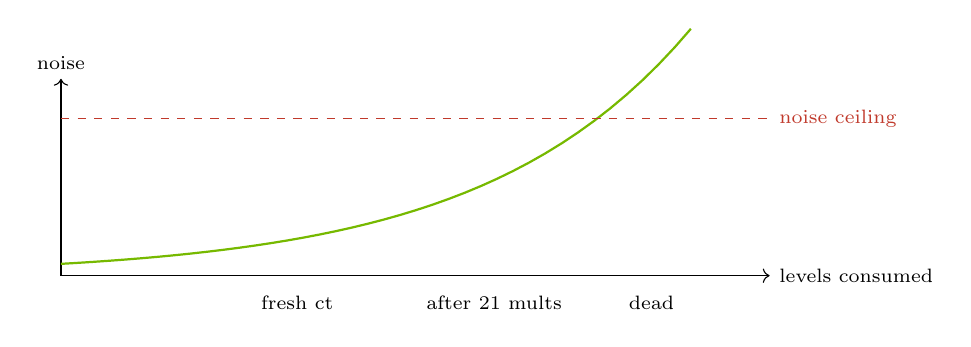
\begin{tikzpicture}[font=\scriptsize]
    \draw[->] (0,0) -- (9,0) node[right] {levels consumed};
    \draw[->] (0,0) -- (0,2.5) node[above] {noise};
    \draw[thick,gpuGreen] plot[domain=0:8,samples=40] (\x, {0.15*exp(0.38*\x)});
    \draw[dashed,accentRed] (0,2.0) -- (9,2.0) node[right] {\color{accentRed}noise ceiling};
    \node at (3,-0.35) {fresh ct};
    \node at (5.5,-0.35) {after 21 mults};
    \node at (7.5,-0.35) {dead};
  \end{tikzpicture}
  \end{center}
  \vspace{0.2em}
  \begin{block}{\textbf{Bootstrapping} = homomorphic decryption-then-encryption}
    \footnotesize
    Evaluate $\mathrm{Dec}$ \emph{as an FHE circuit}, consuming some levels but
    producing a fresh ciphertext of the same message at full level. In CKKS this is
    \textbf{CoeffToSlot $\to$ ModReduce polynomial $\to$ SlotToCoeff}. It costs
    $\sim$10$^5$ kernel launches and \textbf{93\% of our layer runtime}.
  \end{block}
\end{frame}

% ---------------------------------------------------------------------------
\begin{frame}{Transformer operations $\to$ FHE circuits}
  What a plaintext transformer does, and what FHE has to do instead:
  \vspace{0.4em}
  \scriptsize
  \begin{tabular}{@{}p{3.4cm}p{8.1cm}@{}}
    \toprule
    \textbf{Operation} & \textbf{FHE realization} \\
    \midrule
    Linear layer ($W x$) & Plaintext $\times$ ciphertext matmul — cheap, but needs
                           rotations to align operands. \\
    Attention $QK^\top$  & Ciphertext $\times$ ciphertext multiply + relinearization
                           (a key-switch) + rescale. \\
    Softmax              & No "$\exp$" or "$\div$" in FHE! Use a \emph{polynomial approximation}
                           (degree $\sim$60 Chebyshev/Remez), plus many rotations for the
                           denominator sum. \\
    LayerNorm / RMSNorm  & Same story — polynomial for $1/\sqrt{\cdot}$, plus slot reductions. \\
    GELU / SiLU          & Smooth activations $\to$ polynomial approximation
                           (degree $\sim$59). \\
    Residual connection  & Homomorphic addition — essentially free. \\
    \bottomrule
  \end{tabular}
  \normalsize
  \vspace{0.6em}
  \begin{alertblock}{Why this is an HPC workload, not just a crypto one}
    \footnotesize
    Every polynomial approximation consumes multiplicative levels $\Rightarrow$
    bootstraps $\Rightarrow$ thousands of NTTs. A single transformer layer
    triggers 4 bootstraps, each is a $\sim$10-second kernel graph.
  \end{alertblock}
\end{frame}

% ---------------------------------------------------------------------------
\begin{frame}{Security parameters have a scaling cost}
  \begin{block}{The security--performance ladder}
    \footnotesize
    \begin{tabular}{@{}llll@{}}
      \toprule
      $N$ & Noise budget & Use case & Per-op cost \\
      \midrule
      $2^{13}$ & small & toy demos     & milliseconds \\
      $2^{14}$ & medium & some matmuls  & 10s of ms \\
      $2^{15}$ & large  & bootstrap-lite (NEXUS) & seconds \\
      $2^{16}$ & huge   & \alert{bootstrap-at-128-bit-security} & \alert{tens of seconds} \\
      \bottomrule
    \end{tabular}
  \end{block}
  \vspace{0.4em}
  Doubling $N$ doubles polynomial degree, doubles NTT cost ($\mathcal{O}(N \log N)$),
  and \emph{quadruples} key size (larger poly $\times$ more RNS limbs).
  \vspace{0.6em}
  \begin{alertblock}{Why this matters for our story}
    \footnotesize
    NEXUS had to \textbf{lower $N$ from $2^{16}$ to $2^{15}$ for bootstrap}
    ("adjusted for A100 memory"). That's a security downgrade they only accepted
    because their two-server protocol hid it behind parameter-switching.
    \textbf{We run at $2^{16}$ throughout.}
  \end{alertblock}
\end{frame}

% ============================================================================
\section{Related work}
% ============================================================================

\begin{frame}{Where the field stands}
  \begin{columns}[T]
    \begin{column}{0.5\textwidth}
      \textbf{Interactive protocols} (HE + MPC)
      \begin{itemize}
        \item \textsc{Iron}, \textsc{BOLT}, \textsc{BumbleBee}, \textsc{PUMA}
        \item Client and server exchange 10$^4$+ rounds
        \item 60+ GB bandwidth per query
        \item \color{mutedGray}\emph{HPC-hostile: latency-bound}
      \end{itemize}
    \end{column}
    \begin{column}{0.5\textwidth}
      \textbf{Non-interactive (pure FHE)}
      \begin{itemize}
        \item \textsc{NEXUS} (NDSS '25) — 37.3\,s BERT, 4$\times$A100,
              \alert{single node}
        \item \textsc{Cerium} (arXiv '25) — 134\,s Llama3-8B on
              a custom multi-GPU FHE lib (FIDESlib)
        \item \color{mutedGray}\emph{HPC-friendly: one request, no ping-pong}
      \end{itemize}
    \end{column}
  \end{columns}
  \vspace{1em}
  \begin{alertblock}{The gap we attack}
    \small
    NEXUS's protocol is elegant but \emph{single-node}. Cerium is multi-GPU but
    uses a \emph{custom FHE library}. No existing work runs a non-interactive
    FHE transformer on \textbf{multi-node HPC hardware using a mainstream FHE library}.
  \end{alertblock}
\end{frame}

% ---------------------------------------------------------------------------
\begin{frame}{The memory wall at $N{=}65536$}
  \begin{block}{Why NEXUS stopped at one node}
    At the security-required parameter $N{=}65536$:
    \vspace{0.4em}
    \begin{itemize}
      \item One Galois rotation key $= 1.30$ GB on GPU
      \item A full rotation key set (48 keys) $= 62.4$ GB
      \item H100 has 64 GB — \alert{0 MB left for ciphertexts}
    \end{itemize}
    NEXUS's own source: \texttt{logN = 15; // 16 -> 15}
    \footnotesize\color{mutedGray}\emph{"adjusted to satisfy A100 memory constraints"}
  \end{block}
  \pause
  \begin{block}{Existing responses}
    \begin{itemize}
      \item \textsc{NEXUS}: two-server \emph{parameter switching} (ugly, interactive)
      \item \textsc{Cerium}: write a custom FHE library ($\sim$50k lines, FIDESlib)
      \item \textbf{Ours}: treat it as a memory-hierarchy problem
    \end{itemize}
  \end{block}
\end{frame}

% ============================================================================
\section{Our approach: CPU--GPU key streaming}
% ============================================================================

\begin{frame}{The idea — in one picture}
  \begin{center}
  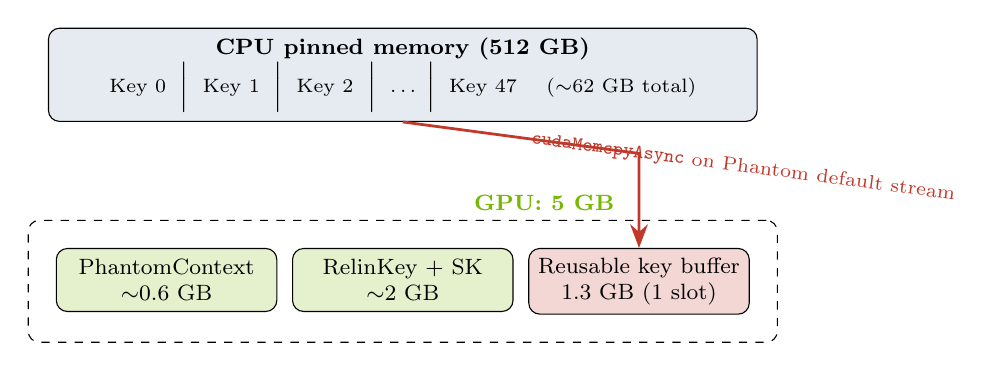
\begin{tikzpicture}[font=\footnotesize,
      box/.style={draw,rounded corners,minimum width=2.8cm,minimum height=0.8cm,align=center},
      bigbox/.style={draw,rounded corners,fill=hpcBlue!10,minimum width=9cm,minimum height=1.1cm,align=center}
    ]
    \node[bigbox] (cpu) {\textbf{CPU pinned memory (512 GB)} \\ {\scriptsize Key 0 $\;\big|\;$ Key 1 $\;\big|\;$ Key 2 $\;\big|\;$ \dots $\;\big|\;$ Key 47 \quad ($\sim$62 GB total)}};

    \node[box,fill=gpuGreen!20,below=1.6cm of cpu, xshift=-3cm] (ctx) {PhantomContext \\ $\sim$0.6 GB};
    \node[box,fill=gpuGreen!20,below=1.6cm of cpu] (rk) {RelinKey + SK \\ $\sim$2 GB};
    \node[box,fill=accentRed!20,below=1.6cm of cpu, xshift=3cm] (slot) {Reusable key buffer \\ 1.3 GB (1 slot)};

    \node[draw,dashed,rounded corners,fit=(ctx)(rk)(slot),inner sep=0.35cm,label=above right:{\color{gpuGreen}\textbf{GPU: 5 GB}}] {};

    \draw[-{Stealth[length=3mm]},line width=1pt,accentRed] (cpu.south) -- ++(3,-0.4)
      node[midway,right,sloped]{\scriptsize \texttt{cudaMemcpyAsync} on Phantom default stream}
      -- (slot.north);
  \end{tikzpicture}
  \end{center}
  \vspace{0.3em}
  \begin{itemize}\footnotesize
    \item Keys live in CPU pinned memory. GPU holds one at a time.
    \item Every rotation asks: \emph{is the right key resident?} Stream if not.
    \item Classic HPC memory-hierarchy pattern — just applied to crypto.
  \end{itemize}
\end{frame}

% ---------------------------------------------------------------------------
\begin{frame}[fragile]{The hook — three lines that rewire everything}
  \begin{lstlisting}
// ckks_evaluator.cuh
inline void rotate_vector(PhantomCiphertext &ct, int step,
                          PhantomGaloisKey &gk, PhantomCiphertext &dest) {
  ensure_key_loaded(step, gk);          //  <-- new
  dest = ::rotate_vector(*context, ct, step, gk);
}
  \end{lstlisting}
  \pause
  \begin{block}{Why this matters to the architecture}
    \begin{itemize}
      \item Every operator (softmax, layer-norm, GELU, bootstrap) calls
            \texttt{rotate\_vector}.
      \item We inherit the \emph{entire} NEXUS operator library without touching it.
      \item $\sim$150 lines of retrofit across 5 Phantom headers, 0 lines
            touched in operator implementations.
    \end{itemize}
  \end{block}
\end{frame}

% ---------------------------------------------------------------------------
\begin{frame}{Phantom retrofit at a glance}
  \scriptsize
  \begin{tabular}{@{}p{4.3cm}p{7.5cm}@{}}
    \toprule
    \textbf{Change} & \textbf{Why it was needed} \\
    \midrule
    \texttt{copy\_to\_host / load\_from\_host} & Serialize a single key's RNS limbs between CPU and GPU. \\
    \texttt{set\_external\_buffers(...)} & Put key in \emph{non-owning} mode — one GPU buffer, many keys. \\
    \texttt{generate\_single\_galois\_key} & Generate keys one at a time (else OOM during setup). \\
    \texttt{setup\_galois\_tool(elts)} & Late permutation-table init without key generation. \\
    \texttt{cuda\_auto\_ptr::owns\_} flag & Avoid double-free when wrapping external buffers. \\
    \bottomrule
  \end{tabular}
  \vspace{1em}
  \begin{block}{Engineering decision}
    \small
    We \textbf{did not fork} Phantom. Five headers touched, all NTT hot-loop
    kernels untouched. We inherit every future Phantom optimization for free.
  \end{block}
\end{frame}

% ---------------------------------------------------------------------------
\begin{frame}{Proof it works}
  \begin{center}
  \begin{tabular}{@{}lr@{}}
    \toprule
    \textbf{Metric (standalone bootstrap, $N{=}65536$, 1$\times$H100)} & \textbf{Value} \\
    \midrule
    Post-bootstrap mean absolute error & $2.25\times10^{-6}$ \alert{(PASS)} \\
    Bootstrap wall time                 & $10.7$ s \\
    GPU memory used                     & $\mathbf{4.93}$ GB / 63.4 GB \\
    CPU memory (Galois keys, pinned)    & $62.4$ GB \\
    Key loads during one bootstrap      & 75 (all successful) \\
    \bottomrule
  \end{tabular}
  \end{center}
  \vspace{0.6em}
  \begin{alertblock}{First result to report here}
    To our knowledge this is the first \emph{single-GPU} run of a CKKS
    bootstrap at $N{=}65536$ using a mainstream FHE library. NEXUS skipped it;
    we don't need to.
  \end{alertblock}
\end{frame}

% ============================================================================
\section{Scaling: multi-GPU and multi-node}
% ============================================================================

\begin{frame}{Multi-GPU: head-level parallelism}
  \begin{block}{Why not split keys across GPUs?}
    We tried. Result: MAE $= 10^{238}$ (FAIL).\\
    \footnotesize
    Root cause: Phantom is \textbf{context-bound}. Each GPU's
    \texttt{PhantomContext} owns its own NTT tables; a ciphertext rotated on
    GPU\,1 cannot be correctly operated on using GPU\,0's NTT representation.
    \normalsize
  \end{block}
  \pause
  \begin{block}{What works: one context per GPU, one head per stream}
    \begin{itemize}\small
      \item One \texttt{std::thread} per GPU.
      \item Each thread builds its own \texttt{PhantomContext}, secret key,
            and CPU key store.
      \item Phantom's \texttt{default\_stream} is \texttt{thread\_local} — CUDA ops
            auto-route to the right GPU.
      \item Heads distributed round-robin: GPU\,$g$ gets heads
            $\{g, g{+}G, g{+}2G,\dots\}$.
    \end{itemize}
  \end{block}
\end{frame}

% ---------------------------------------------------------------------------
\begin{frame}{Multi-node: MPI scatter/gather}
  \begin{center}
  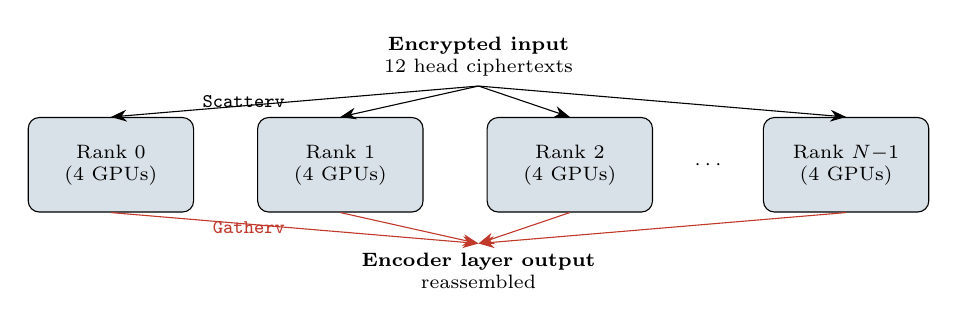
\begin{tikzpicture}[font=\scriptsize,
      rank/.style={draw,rounded corners,fill=hpcBlue!15,minimum width=2.1cm,minimum height=1.2cm,align=center}]
    \node[rank] (r0) {Rank 0 \\ (4 GPUs)};
    \node[rank,right=0.8cm of r0] (r1) {Rank 1 \\ (4 GPUs)};
    \node[rank,right=0.8cm of r1] (r2) {Rank 2 \\ (4 GPUs)};
    \node[right=0.4cm of r2] (dots) {$\cdots$};
    \node[rank,right=0.4cm of dots] (rN) {Rank $N{-}1$ \\ (4 GPUs)};

    \node[above=1.0cm of $(r0)!0.5!(rN)$, align=center]
      (input) {\textbf{Encrypted input} \\ 12 head ciphertexts};
    \draw[-{Stealth[length=2mm]}] (input.south) -- (r0.north) node[midway,left]{\texttt{Scatterv}};
    \draw[-{Stealth[length=2mm]}] (input.south) -- (r1.north);
    \draw[-{Stealth[length=2mm]}] (input.south) -- (r2.north);
    \draw[-{Stealth[length=2mm]}] (input.south) -- (rN.north);

    \node[below=1.0cm of $(r0)!0.5!(rN)$, align=center]
      (out) {\textbf{Encoder layer output} \\ reassembled};
    \draw[-{Stealth[length=2mm]},accentRed] (r0.south) -- (out.north) node[midway,left]{\texttt{Gatherv}};
    \draw[-{Stealth[length=2mm]},accentRed] (r1.south) -- (out.north);
    \draw[-{Stealth[length=2mm]},accentRed] (r2.south) -- (out.north);
    \draw[-{Stealth[length=2mm]},accentRed] (rN.south) -- (out.north);
  \end{tikzpicture}
  \end{center}
  \vspace{0.3em}
  \begin{itemize}\small
    \item 12 heads / $N$ ranks $\Rightarrow$ uneven chunks $\Rightarrow$
          \texttt{MPI\_Scatterv} / \texttt{Gatherv} are the natural fit.
    \item Measured scatter + gather: \textbf{0.5--0.6 s, independent of node count}.
  \end{itemize}
\end{frame}

% ============================================================================
\section{Experimental setup}
% ============================================================================

\begin{frame}{Hardware: MareNostrum 5 (BSC)}
  \begin{columns}[T]
    \begin{column}{0.55\textwidth}
      \textbf{ACC partition}
      \begin{itemize}\small
        \item 1120 nodes, 4$\times$NVIDIA H100 64\,GB SXM5 each
        \item 2$\times$Intel Xeon Platinum 8460Y+ (56 cores $\times$ 2)
        \item 512 GB DDR5 per node
        \item Slingshot-11 interconnect (200 Gbps/link, 4 links/node)
        \item SLURM / QOS \texttt{acc\_debug}, project \texttt{etur02}
      \end{itemize}
    \end{column}
    \begin{column}{0.45\textwidth}
      \textbf{Software stack}
      \begin{itemize}\small
        \item CUDA 12.8, NCCL 2.24.3, OpenMPI 4.1.5
        \item Phantom FHE (retrofitted)
        \item CKKS $N{=}65536$, 128-bit security,
              Hamming-weight sparse key = 192
        \item Build: \texttt{cmake} + \texttt{make -j16}
      \end{itemize}
    \end{column}
  \end{columns}
  \vspace{0.6em}
  \begin{block}{Why MN5 and not AWS?}
    \footnotesize
    AWS-granted quota: 8 vCPU on P-instances $\Rightarrow$ p4d.24xlarge blocked.
    MN5 gave us up to 8 nodes = 32$\times$H100 with InfiniBand-class fabric, SLURM QOS,
    and a pre-allocated project directory — a \emph{real} HPC platform for the
    experiment.
  \end{block}
\end{frame}

% ============================================================================
\section{Results}
% ============================================================================

\begin{frame}{Strong scaling — BERT, $N{=}65536$, 12 heads}
  \begin{center}
  \begin{tabular}{@{}lrrrrr@{}}
    \toprule
    \textbf{Config} & \textbf{Nodes} & \textbf{GPUs} &
      \textbf{Total} & \textbf{Compute (max)} & \textbf{Speed-up} \\
    \midrule
    1-node & 1 & 4  & 238.7 s & 191.4 s & $1.00\times$ \\
    2-node & 2 & 8  & 183.7 s & 129.3 s & $1.30\times$ \\
    4-node & 4 & 16 & 146.3 s &  95.4 s & $1.63\times$ \\
    8-node & 8 & 32 & \textbf{103.5 s} & \textbf{55.2 s} & $\mathbf{2.31\times}$ \\
    \bottomrule
  \end{tabular}
  \end{center}
  \vspace{0.4em}
  \begin{itemize}\small
    \item Scatter/gather: \textbf{0.51--0.63 s} at all configs ($<0.6$\% of total).
    \item Setup ($\sim$47 s/node) is constant — dominates small configs.
    \item Sub-linear: 12 heads $\not\equiv 0 \pmod{16, 32}$ $\Rightarrow$ load imbalance bounded by slowest GPU.
  \end{itemize}
\end{frame}

% ---------------------------------------------------------------------------
\begin{frame}{Strong scaling — LLaMA, $N{=}65536$, 12 heads}
  \begin{center}
  \begin{tabular}{@{}lrrrrr@{}}
    \toprule
    \textbf{Config} & \textbf{Nodes} & \textbf{GPUs} &
      \textbf{Total} & \textbf{Compute (max)} & \textbf{Speed-up} \\
    \midrule
    1-node & 1 & 4  & 249.6 s & 198.9 s & $1.00\times$ \\
    2-node & 2 & 8  & 208.6 s & 152.2 s & $1.20\times$ \\
    4-node & 4 & 16 & 122.5 s &  74.4 s & $2.04\times$ \\
    8-node & 8 & 32 & \textbf{103.0 s} & \textbf{55.8 s} & $\mathbf{2.42\times}$ \\
    \bottomrule
  \end{tabular}
  \end{center}
  \vspace{0.4em}
  \begin{itemize}\small
    \item Scatter/gather: \textbf{0.31--0.62 s} ($<0.6$\% of total).
    \item LLaMA scales more aggressively at 4-node: \emph{faster} than BERT
          (122.5 s vs 146.3 s) because per-head compute time is higher,
          so 1-head bound is hit sooner.
    \item At 8-node both architectures converge to $\sim$103 s —
          dominated by setup + single-head bootstrap (4$\times\sim$13.5 s).
  \end{itemize}
\end{frame}

% ---------------------------------------------------------------------------
\begin{frame}{BERT vs LLaMA — side-by-side scaling}
  \begin{center}
  \begin{tabular}{@{}lrrrr@{}}
    \toprule
    & \multicolumn{2}{c}{\textbf{Total wall-time (s)}} & \multicolumn{2}{c}{\textbf{Speedup vs 1-node}} \\
    \cmidrule(lr){2-3}\cmidrule(lr){4-5}
    \textbf{Config} & BERT & LLaMA & BERT & LLaMA \\
    \midrule
    1-node / 4 GPUs  & 238.7 & 249.6 & $1.00\times$ & $1.00\times$ \\
    2-node / 8 GPUs  & 183.7 & 208.6 & $1.30\times$ & $1.20\times$ \\
    4-node / 16 GPUs & 146.3 & \textbf{122.5} & $1.63\times$ & $\mathbf{2.04\times}$ \\
    8-node / 32 GPUs & 103.5 & \textbf{103.0} & $2.31\times$ & $\mathbf{2.42\times}$ \\
    \bottomrule
  \end{tabular}
  \end{center}
  \vspace{0.5em}
  \begin{alertblock}{Key insight}
    \small
    At 8-node/32-GPU both architectures converge to the \textbf{same wall time}
    ($\sim$103 s). The bottleneck is universal: 4 bootstraps at
    $\sim$13.5 s each, independent of architecture.\\[0.3em]
    \textbf{Platform, not architecture, sets the floor.}
  \end{alertblock}
\end{frame}

% ---------------------------------------------------------------------------
\begin{frame}{Where is time actually spent? (Nsight, 1-node / 4-GPU)}
  \scriptsize
  \begin{center}
  \begin{tabular}{@{}lrrr@{}}
    \toprule
    \textbf{Top CUDA kernels} & \textbf{Total (ms)} & \textbf{Avg (\textmu s)} & \textbf{\% GPU time} \\
    \midrule
    \texttt{fnwt\_radix8\_phase2\_fuse\_moddown} (fused NTT+moddown) & 620\,776 & 51.8 & 2.3 \\
    \texttt{sample\_uniform\_poly} (key-switch randomness)           & 546\,691 & 59.1 & 2.0 \\
    \texttt{multiply\_and\_add\_negate\_rns\_poly}                   & 476\,822 & 51.5 & 1.8 \\
    \texttt{special\_ifft\_base} (CoeffToSlot FFT)                   & 338\,812 & 13.5 & 1.3 \\
    \texttt{decompose\_array\_uint64}                                & 301\,563 & 12.0 & 1.1 \\
    \bottomrule
  \end{tabular}
  \vspace{0.6em}

  \begin{tabular}{@{}lrr@{}}
    \toprule
    \textbf{Memory traffic} & \textbf{Total (MB)} & \textbf{Count} \\
    \midrule
    H$\to$D (key streaming!) & 5\,277\,008 & 533 k \\
    D$\to$D (intra-kernel)   & \phantom{5\,}3\,884\,501 & 188 k \\
    D$\to$H (output only)    & \phantom{5\,277\,}365\,485 &  34 k \\
    \bottomrule
  \end{tabular}
  \end{center}
  \vspace{0.4em}
  \normalsize
  No single kernel over 3\% — this is a \textbf{breadth-first} workload.
  Streaming traffic (5.3 TB) is real but \emph{overlapped} with compute.
\end{frame}

% ---------------------------------------------------------------------------
\begin{frame}{Granular breakdown: one BERT encoder layer}
  \scriptsize
  \begin{columns}[T]
    \begin{column}{0.48\textwidth}
      \textbf{Per-operation (12 heads summed)}
      \vspace{0.2em}
      \begin{tabular}{@{}lrr@{}}
        \toprule
        Op & Time & \% \\
        \midrule
        Bootstrap \#1 & 142.2 s & 23.8 \\
        Bootstrap \#4 & 142.7 s & 23.8 \\
        Bootstrap \#2 & 138.1 s & 23.1 \\
        Bootstrap \#3 & 136.0 s & 22.7 \\
        LayerNorm \#2 & \phantom{1}13.6 s & 2.3 \\
        LayerNorm \#1 & \phantom{1}12.9 s & 2.2 \\
        Softmax       & \phantom{10}9.3 s & 1.6 \\
        QKV MatMul    & \phantom{10}1.4 s & 0.2 \\
        GELU          & \phantom{10}1.1 s & 0.2 \\
        (all other MatMuls) & \phantom{100}1.2 s & 0.2 \\
        \midrule
        \textbf{Total work} & \textbf{598.5 s} & \textbf{100} \\
        \bottomrule
      \end{tabular}
    \end{column}
    \begin{column}{0.5\textwidth}
      \textbf{Category rollup}
      \vspace{0.4em}

      \begin{tabular}{@{}lr@{}}
        \toprule
        Category & \% \\
        \midrule
        Bootstraps (4$\times$)              & \textbf{93.4} \\
        Non-linear (Softmax, LN, GELU)      & 6.2 \\
        MatMuls (6$\times$)                 & 0.4 \\
        \bottomrule
      \end{tabular}

      \vspace{1em}
      \begin{block}{What this tells an HPC audience}
        \footnotesize
        \begin{itemize}
          \item Bootstrap is \emph{the} target.
          \item Streaming overhead is already invisible (MatMuls 0.4\%).
          \item Roofline-style analysis would show bootstrap as memory-bound
                at these NTT sizes.
        \end{itemize}
      \end{block}
    \end{column}
  \end{columns}
\end{frame}

% ---------------------------------------------------------------------------
\begin{frame}{Framework is architecture-agnostic: LLaMA layer}
  \scriptsize
  \textbf{Single-node (1-node / 4-GPU) profile comparison:}
  \vspace{0.2em}
  \begin{tabular}{@{}lrrr@{}}
    \toprule
    Metric & BERT & LLaMA & $\Delta$ \\
    \midrule
    Wall-clock total         & 238.7 s & 249.6 s & +4.6\% \\
    Summed work (12 heads)   & 598.5 s & 678.3 s & +13.3\% \\
    Average bootstrap        & 11.65 s & 13.17 s & +13.1\% \\
    Non-linear total         & \phantom{1}36.9 s & \phantom{1}40.6 s & +10.0\% \\
    MatMul total (6× vs 7×)  & \phantom{10}2.6 s & \phantom{10}3.5 s & +36.2\% \\
    RoPE + gate$\odot$up     & — & \phantom{10}2.2 s & n/a \\
    \bottomrule
  \end{tabular}
  \vspace{0.6em}
  \normalsize
  \begin{block}{HPC-relevant takeaways}
    \footnotesize
    \begin{itemize}
      \item Zero changes to Phantom, key-streaming, multi-GPU, or MPI layer —
            swap a \texttt{.cu} file, rebuild, submit.
      \item LLaMA's SwiGLU extra mul-level raises bootstrap cost by 13\%,
            not the RoPE (0.3\%) or the extra matmul (0.1\%).
      \item At 8-node/32-GPU both architectures converge to $\sim$103 s —
            the platform sets the floor, not the architecture.
    \end{itemize}
  \end{block}
\end{frame}

% ---------------------------------------------------------------------------
\begin{frame}{Design discussion: MPI vs NCCL vs NVSHMEM}
  \begin{block}{Our workload inter-node}
    One scatter + one gather \emph{per encoder layer}. No in-loop collectives.
    Chunks are \emph{uneven} (12 heads $\div$ $N$ nodes).
  \end{block}
  \pause
  \begin{block}{Why MPI wins here}
    \small
    \begin{itemize}
      \item \texttt{Scatterv}/\texttt{Gatherv} handle uneven chunks natively.
      \item Measured cost: 0.5\% of total. Even a 10$\times$ faster transport buys 0.05\%.
      \item NCCL is optimized for fixed-size collectives in tight loops (think
            gradient all-reduce). Overkill and awkward here.
      \item We \emph{do} use NCCL for \textbf{intra-node} key-switching
            micro-benchmarks where bandwidth actually matters.
    \end{itemize}
  \end{block}
  \pause
  \begin{alertblock}{HPC engineering principle}
    Don't pay for a lower-level transport when communication is already
    in the noise.
  \end{alertblock}
\end{frame}

% ============================================================================
\section{Discussion and future work}
% ============================================================================

\begin{frame}{What we did vs.\ what's left}
  \begin{columns}[T]
    \begin{column}{0.5\textwidth}
      \textbf{\color{gpuGreen}Done}
      \begin{itemize}\small
        \item First $N{=}65536$ bootstrap on one H100 (mainstream library)
        \item End-to-end BERT encoder layer, no parameter switching
        \item 8-node / 32-GPU scaling on MN5 (2.31$\times$)
        \item Nsight + granular per-op profile
        \item LLaMA-style cross-architecture comparison
        \item MPI + thread-per-GPU scaling pattern
      \end{itemize}
    \end{column}
    \begin{column}{0.5\textwidth}
      \textbf{\color{accentRed}Open}
      \begin{itemize}\small
        \item LRU key cache on GPU\\
              \footnotesize(bootstrap reuses keys predictably — could cut streaming
              cost 10--20$\times$)
        \normalsize
        \item Full 12-layer BERT (we ran 1 layer;
              the block repeats)
        \item Port hook to FIDESlib when Cerium releases
        \item Fused CoeffToSlot kernel (the current Nsight hot-spot)
      \end{itemize}
    \end{column}
  \end{columns}
\end{frame}

% ---------------------------------------------------------------------------
\begin{frame}{Take-aways for HPC researchers}
  \begin{enumerate}
    \item \textbf{Crypto is an HPC workload.} NTT-heavy, memory-heavy,
          bootstrap-dominated. All standard HPC tools apply: Nsight, NCCL,
          MPI, SLURM, roofline thinking.
    \item \textbf{Memory-hierarchy tricks port straight across.}
          CPU$\to$GPU staging is not fancy in graphics or scientific computing;
          it's new in FHE because keys are enormous and the library world
          hasn't caught up.
    \item \textbf{Avoid rewriting the kernel library.} Intercept at the operator level.
          Three lines of hook + a retrofit of 150 lines bought us an 8-node-capable system.
    \item \textbf{Profile before you optimize.} Bootstrap is 93\%; anything else
          is rounding error.
    \item \textbf{Pick the transport the workload asks for.}
          MPI for once-per-layer scatter. NCCL for inside hot loops. Don't default to the fastest.
  \end{enumerate}
\end{frame}

% ---------------------------------------------------------------------------
\begin{frame}[plain]
  \begin{center}
    {\Huge Thank you}\\[1em]
    {\Large Questions?}\\[2em]
    \small Halil İbrahim Kanpak — Koç University, Comp390 \\
    Advisor: Prof.\ Didem Unat
  \end{center}
\end{frame}

% ============================================================================
\appendix
\section*{Backup slides}
% ============================================================================

\begin{frame}{Backup: CKKS parameter set used}
  \scriptsize
  \begin{tabular}{@{}lr@{}}
    \toprule
    Parameter & Value \\
    \midrule
    Polynomial degree $N$                & $2^{16}$ \\
    Sparse slots                         & $2^{14}$ \\
    Log of scale $\log_2 \Delta$         & 46 \\
    Log of prime $\log_2 q_0$            & 51 \\
    Special modulus $\log_2$             & 51 \\
    Main multiplicative levels           & 21 \\
    Bootstrap levels                     & 14 \\
    Total chain depth                    & 35 \\
    Hamming weight of secret key         & 192 \\
    Claimed security                     & 128-bit \\
    \bottomrule
  \end{tabular}
  \vspace{0.8em}
  \normalsize
  Same parameter set as NEXUS for non-bootstrap operations.
  We additionally \emph{run} bootstrap at this $N$; NEXUS does not.
\end{frame}

\begin{frame}{Backup: per-GPU memory budget}
  \scriptsize
  \begin{tabular}{@{}lr@{}}
    \toprule
    Item & GPU memory \\
    \midrule
    PhantomContext + NTT tables       & 0.61 GB \\
    Secret key                        & 0.32 GB \\
    Public key                        & 0.63 GB \\
    Relinearization key               & 0.94 GB \\
    One streaming Galois-key buffer   & 1.30 GB \\
    Working ciphertexts + intermediates & $\sim$1.2 GB \\
    \midrule
    \textbf{Peak} (measured)          & \textbf{4.93 GB} / 63.4 GB \\
    \textbf{"Naive" all-keys resident} & 63.4 GB $\Rightarrow$ OOM \\
    \bottomrule
  \end{tabular}
\end{frame}

\begin{frame}{Backup: failed experiment — multi-GPU key distribution}
  \begin{block}{What we tried first}
    Split 48 Galois keys across 2 GPUs (24 each), transfer ciphertexts with
    \texttt{cudaMemcpyPeer}, run key-switching on the GPU that owns the key.
  \end{block}
  \pause
  \begin{alertblock}{Outcome}
    $\textrm{MAE} = 10^{238}$ — catastrophic divergence after one bootstrap.
  \end{alertblock}
  \pause
  \begin{block}{Root cause}
    \footnotesize
    Phantom's \texttt{PhantomContext} owns \emph{GPU-local} NTT tables and
    Galois-permutation tables. Ciphertexts carry a \texttt{parms\_id\_} hash
    that matches across GPUs, but the underlying GPU pointers don't. Operations
    silently use the \emph{wrong} NTT representation, accumulating exponentially.
  \end{block}
  \pause
  \begin{block}{Lesson}
    \small
    Cross-context transfer is only safe if the FHE library is designed for it
    (Cerium's FIDESlib does this; mainstream libraries don't).
    CPU streaming sidesteps the problem entirely.
  \end{block}
\end{frame}

\begin{frame}{Backup: NVIDIA Nsight command used}
  \begin{lstlisting}[language=bash]
nsys profile \
  --trace=cuda,nvtx,osrt \
  --cuda-memory-usage=true \
  --output=nsight_n65k_4gpu \
  ${BIN}/bert_encoder_multigpu_n65536 \
    --n-gpus 4 --heads 12 --hidden 64 --inner 64 --seq-len 16

nsys stats \
  --report gputrace,gpukernsum,gpumemtimesum,gpumemsizesum \
  nsight_n65k_4gpu.nsys-rep
  \end{lstlisting}
  \small
  Report archived at\\
  \texttt{/gpfs/projects/etur02/hkanpak/logs/nsight\_n65k\_4gpu.nsys-rep}
\end{frame}

\begin{frame}{Backup: bibliography pointers}
  \scriptsize
  \begin{itemize}
    \item Zhang et al., \textbf{NEXUS}: Secure and Non-Interactive Transformer
          Inference on Encrypted Data. \emph{NDSS} 2025.
    \item Jayashankar et al., \textbf{Cerium}: A Scalable Multi-GPU Framework
          for Encrypted Large-Model Inference. arXiv:2512.11269, 2025.
    \item Jayashankar et al., \textbf{Cinnamon}: A Framework for Scale-Out
          Encrypted AI. \emph{ASPLOS} 2025.
    \item Yang et al., \textbf{Phantom}: A CUDA-Accelerated FHE Library for
          CKKS/BFV. GitHub: \texttt{encryptorion-lab/phantom-fhe}.
    \item Cheon et al., \textbf{CKKS}: Homomorphic Encryption for Arithmetic
          of Approximate Numbers. \emph{ASIACRYPT} 2017.
  \end{itemize}
\end{frame}

\end{document}
